\chapter{Installation}

Before installing ClockAlarm some requirements have to be fulfilled: the
installed Python version should be at least 3.6 and the following packages have
to be installed:

\begin{itemize}
    \item pygame >= 1.9.3
    \item PyQt5 >= 5.8.2 
    \item sip >= 4.19.2
    \item tinydb >= 3.2.2 
\end{itemize}

This can be done with one command: \texttt{pip3 install pygame pyqt5 sip tinydb}.
The repository can be cloned: \texttt{git clone
https://github.com/BFH-BTI7301-project1/ClockAlarm.git}.
The program can finally be run using: \texttt{python3 bin/clockalarm}.

\begin{figure}[h]
    \centering
    \caption{ClockAlarm main window}
    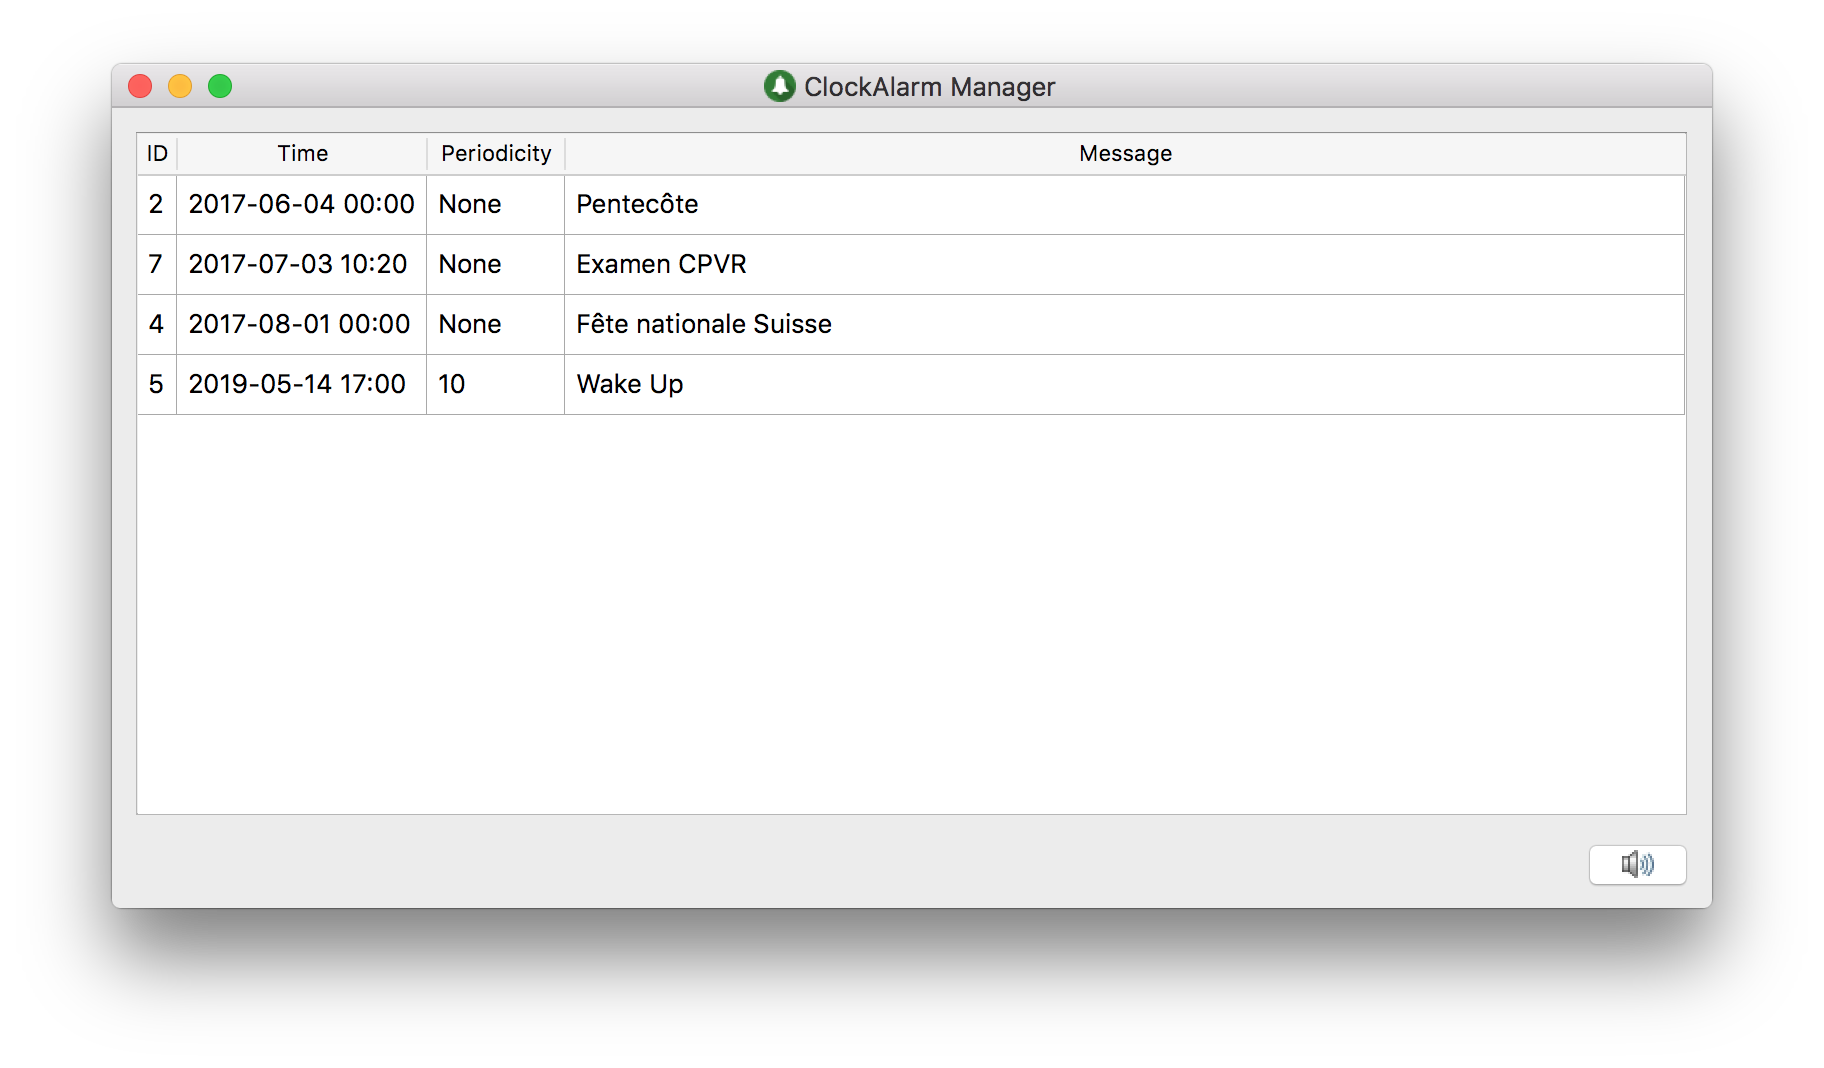
\includegraphics[width=0.9\textwidth]{main_window.png}
\end{figure}

